%% ------------------------------------------------------------------------- %%
\chapter{Melhorias ao Stoa}
\label{cap:melhorias}

    As 10 funcionalidades selecionadas com base na priorização individual de cada grupo, como descrito na seção ~\ref{sec:priorizacao}, foram documentadas para serem avaliadas detalhadamente quanto à usabilidade e, em seguida, melhoradas. Neste capítulo serão descritas soluções encontradas para algumas falhas de usabilidade presentes na lista selecionada, seguindo a seguinte estrutura: cada seção representará uma funcionalidade que possui falhas e será dividida em duas partes, problema e solução. As outras funcionalidades ainda estão em estudo detalhado para melhoria quanto à usabilidade, de modo que ainda não foram apresentadas soluções definitivas sobre elas. 
%cada section será uma das funcionalidades melhoradas%


\section{Quem somos (link no rodapé)}
\label{sec:quem-somos}
    \begin{itemize}
    \item Problema:\\
    É muito comum, ao ingressar em um sistema desconhecida pelo usuário, que ele busque por páginas com informações sobre o sistema para melhor entender seus objetivos e funcionalidades. Com a rede acadêmica Stoa, esse fenômeno é observado; há \emph{links} no rodapé de todas as páginas indicando ao usuário que este pode se informar sobre a rede ou colaborar com ela. Porém, ao clicar nos atalhos do rodapé, como o "Quem somos", há uma quebra na expectativa do usuário, pois ele é redirecionado à mesma página.

    \item Solução:\\
    Para todos os \emph{links} do rodapé, a solução é bem simples, mas um pouco trabalhosa: basta associar uma página do Stoa a cada um e preenchê-la com as informações corretas, ou redirecionar o atalho a uma página já existente.
    
    No caso do \emph{link} "Quem somos", deve-se criar uma página apresentando a história e objetivos do Stoa, informando principalmente como e porque a rede foi criada e quais os propósitos atuais dela.
    \end{itemize}

\section{Google Analytics}
    \begin{itemize}
    \item Problema:\\
    A ferramenta \emph{Google Analytics} é uma ótima maneira de realizar estatísticas sobre acesso e visualização de conteúdos próprios, além de outras funções. Com esta pesquisa, descobriu-se que há muitos usuários do Stoa interessados por essa funcionalidade, mas que desconheciam até o momento da pesquisa a existência desta funcionalidade no Stoa. Outros, ainda, não utilizam esta ferramenta atualmente por não entenderem bem seu funcionamento, deixando, assim, de clicar no atalho para ela.

    \item Solução:\\
    Para esta funcionalidade ser utilizada com mais frequência e corretude, é necessário aumentar a visibilidade da ferramenta, exibindo-a com mais destaque nas páginas em que ela pode ser utilizada, e incluir uma explicação clara e concisa sobre seu funcionamento, para que usuários que nunca a  utilizaram possam fazê-lo com propriedade.
    \end{itemize}

%% ------------------------------------------------------------------------- %%
%\section{Fundamentos}\index{�rea do trabalho!fundamentos}
%\label{sec:fundamentos}


%% ------------------------------------------------------------------------- %%
%%\subsection{�cidos Nucl�icos}\index{�cido!nucl�ico}\index{nucleot�deos}
%%\label{sec:acidos_nucleicos}

%Na Figura~\ref{fig:humanbeta} texto texto texto texto 

%\begin{figure}[!h]
%  \centering
%  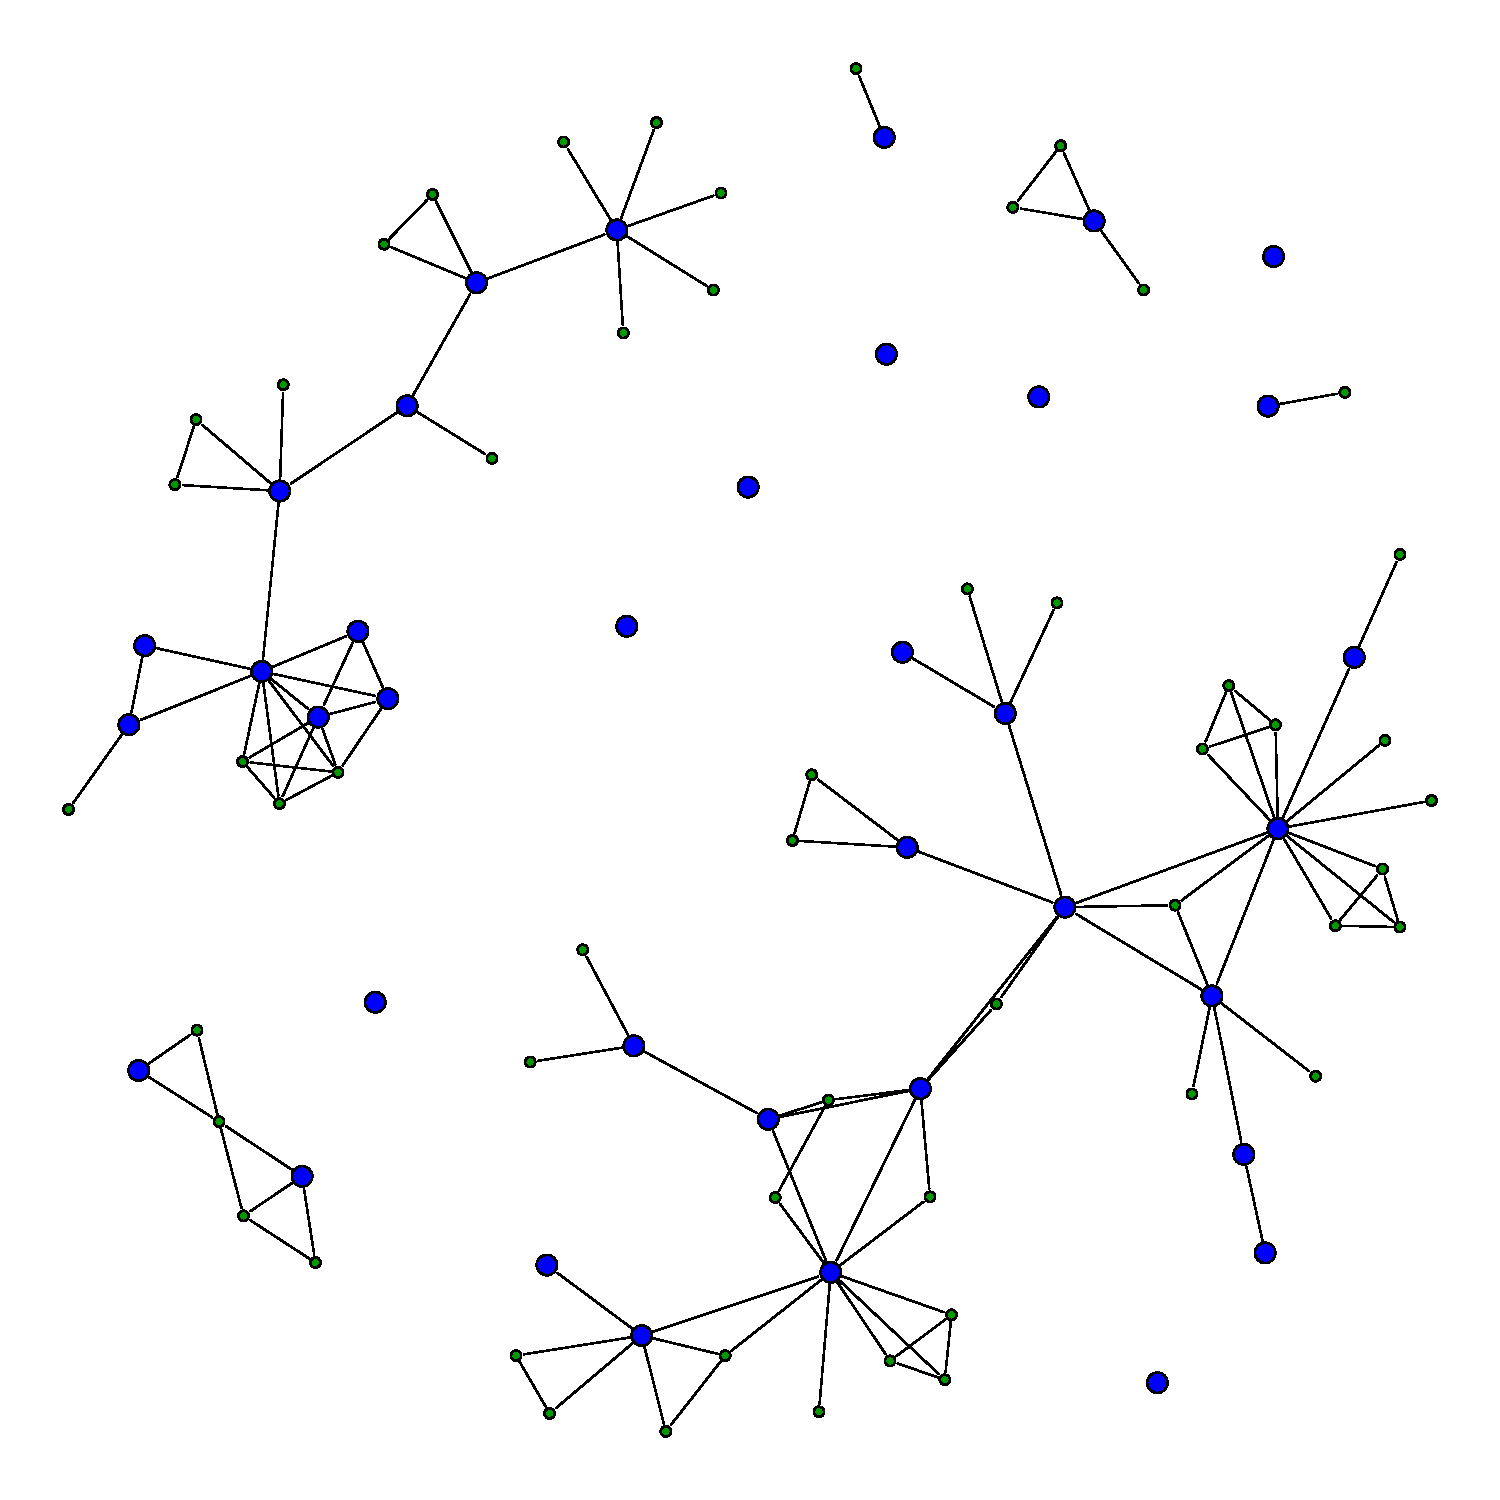
\includegraphics[width=.40\textwidth]{graph} 
%  \caption{Descri��o da figura mostrada.}
%  \label{fig:humanbeta} 
%\end{figure}

%% ------------------------------------------------------------------------- %%
%\subsection{Amino�cidos}\index{�cido!amino|(}
%\label{sec:amino_acidos}

%\begin{table}[!t]
%\begin{center}
%    \begin{tabular}{c|c|l}
%	 \hline
%	 C�digo & Abreviatura & Nome completo \\ \hline
%     \texttt{A} & Ala & Alanina \\
%     \texttt{C} & Cys & Ciste�na \\
%     ...        & ... & ... \\
%     \texttt{W} & Trp & Tiptofano \\
%     \texttt{Y} & Tyr & Tirosina \\ \hline
%    \end{tabular}
%  \caption{C�digos, abreviaturas e nomes dos amino�cidos.}
%  \label{tab:amino_acidos}
%\end{center}
%\end{table}
%\index{�cido!amino|)}


%% ------------------------------------------------------------------------- %%
%\section{Exemplo de C�digo-Fonte em Java}
%\label{sec:exemplo_codigo_fonte}
%Texto texto texto texto texto texto texto texto texto texto texto texto texto

% Foi utilizado o pacote listing para formatar c�digo fonte
% http://ctan.org/tex-archive/macros/latex/contrib/listings/listings.pdf
% Veja no preambulo do arquivo tese-exemplo.tex os par�metros de configura��o.

%\begin{lstlisting}[frame=trbl]
%    for(i = 0; i < 20; i++)
%    {
%        // Coment�rio 
%        System.out.println("Mensagem...");
%    }
%\end{lstlisting}

